

%*----------- SLIDE -------------------------------------------------------------
\begin{frame}[c]{Objetivo}
  \framesubtitle{Da apresentação}
  \transdissolve[duration=0.5]

  \begin{center}
    \Wider{
      \begin{shaded}
        \begin{center}
          \vspace*{0.5cm}
          \resizebox{!}{0.6cm}{%
            \color{black} Entendimento do artigo
          }
        \end{center}
      \end{shaded}
    }
  \end{center}


  %*----------- notes
  \note[item]{Notes can help you to remember important information. Turn on the notes option.}
\end{frame}

%-
%*----------- SLIDE -------------------------------------------------------------

\begin{frame}[t]{Introdução}
  \framesubtitle{O problema}
  \transdissolve[duration=0.5]
  Baixa precisão no comportamento do robô.

  \begin{columns}[t]
    \column{.6\linewidth}
      \begin{figure}
        \includemedia[
          totalheight=0.5\linewidth,
          activate=pageopen,
          passcontext,
          %transparent,
          addresource=./Source/gifs/atlas-jump.wmv,
          flashvars={
            source=./Source/gifs/atlas-jump.wmv
            &autoPlay=true
            &autoRewind=true
            &loop=true}
            ]{\fbox{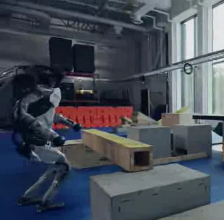
\includegraphics{Source/gifs/atlas-jump.png}}}{VPlayer.swf}
          \caption{Expectativa \cite{BostonDynamicsPartners}} %FIXME: slides não estão numerando as figuras
      \end{figure}
    \column{.6\linewidth}
    \begin{center}
      %\centerline{
      \begin{figure}
        \includemedia[
          totalheight=0.5\linewidth,
        activate=pageopen,
        passcontext,
        %transparent,
        addresource=./Source/gifs/atlas-fail.wmv,
        flashvars={
          source=./Source/gifs/atlas-fail.wmv
          &autoPlay=true
          &autoRewind=true
          &loop=true}
          ]{\fbox{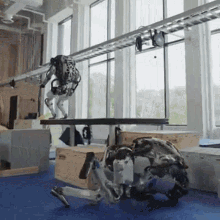
\includegraphics{Source/gifs/atlas-fail.png}}}{VPlayer.swf}
        \caption{Realidade \cite{BostonDynamicsFails}}
      \end{figure}
    \end{center}
  \end{columns}
  %*----------- notes
  \note[item]{Notes can help you to remember important information. Turn on the notes option.}
\end{frame}

%*----------- SLIDE -------------------------------------------------------------
\begin{frame}[t]{Introdução}
  \framesubtitle{O robô utilizado}
  \transdissolve[duration=0.5]

  \begin{figure}[ht!]
    \begin{subfigure}[b]{0.3\textwidth}
      \centering
      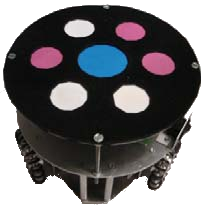
\includegraphics[width=\textwidth]{Three_wheeled_robot.png}
      % \roundpic[xshift=0cm,yshift=0cm]{4.5cm}{4.5cm}{Three_wheeled_robot.png}
      \caption{Roda convencional.}
      \label{fig:3_wheels_robot}
    \end{subfigure}
    ~
    \begin{subfigure}[b]{0.3\textwidth}
      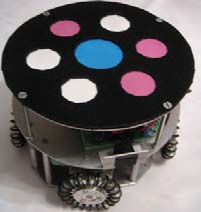
\includegraphics[width=\textwidth]{four_wheeled_robot.png}
      % \roundpic[xshift=0cm,yshift=0cm]{4.5cm}{4.5cm}{four_wheeled_robot.png}
      \caption{Quatro rodas.}
      \label{fig:4_wheels_robot}
    \end{subfigure}
    
  \caption{Plataforma utilizada para comparar às duas configurações. \cite{Oliveira2008}}
  \end{figure}
  
  %*----------- notes
  \note[item]{Notes can help you to remember important information. Turn on the notes option.}
\end{frame}

%*----------- SLIDE -------------------------------------------------------------
\begin{frame}[t]{Introdução}
  \framesubtitle{}
  \transdissolve[duration=0.5]

  \begin{figure}[ht!]
    \centering
    \begin{subfigure}[b]{0.28\textwidth}
      \centering
      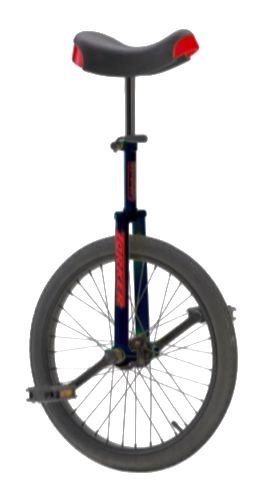
\includegraphics[width=0.7\textwidth]{connventional_wheel.png}
      % \roundpic[xshift=0cm,yshift=0cm]{4.5cm}{4.5cm}{Three_wheeled_robot.png}
      \caption{Roda convencional.}
      \label{fig:Conventional_wheel}
    \end{subfigure}
    ~
    \begin{subfigure}[b]{0.28\textwidth}
      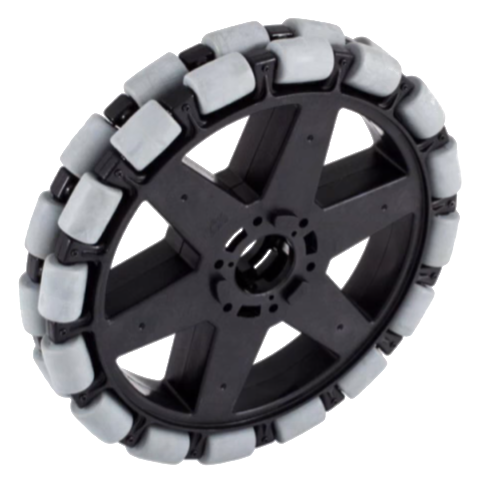
\includegraphics[width=\textwidth]{omniwheel.png}
      % \roundpic[xshift=0cm,yshift=0cm]{4.5cm}{4.5cm}{four_wheeled_robot.png}
      \caption{Omniwheel.}
      \label{ominiwheel}
    \end{subfigure}
    ~
    \begin{subfigure}[b]{0.28\textwidth}
      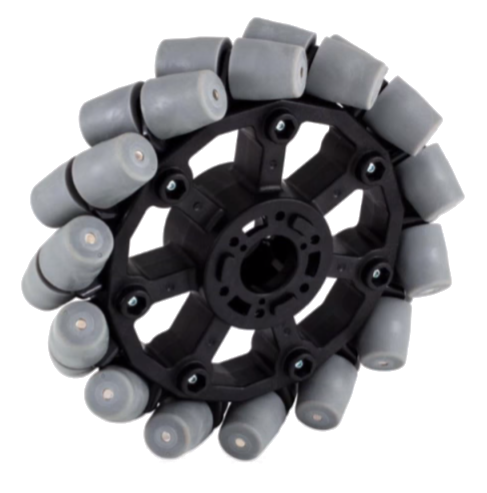
\includegraphics[width=\textwidth]{mecanum_Whell.png}
      % \roundpic[xshift=0cm,yshift=0cm]{4.5cm}{4.5cm}{four_wheeled_robot.png}
      \caption{Roda Mecanum.}
      \label{mecanum_wheel}
    \end{subfigure}
    
  \caption{Tipos de rodas.}
  \end{figure}
  
  %*----------- notes
  \note[item]{Notes can help you to remember important information. Turn on the notes option.}
\end{frame}

%-
%*----------- SLIDE -------------------------------------------------------------
\begin{frame}[t]{Introdução}
  \framesubtitle{As causas elencadas}
  \transdissolve[duration=0.5]
  \begin{enumerate}
    \item Modelo dinâmico incompleto.
    \begin{enumerate}
      \item Dificuldade em modelar os atritos internos.
    \end{enumerate}

    \item Parâmetros imprecisos (específico).
    \begin{enumerate}
      \item Coeficientes de atrito.
      \item Momento inercial.
      \item Constantes dos motores.
    \end{enumerate}
  \end{enumerate}

  %*----------- notes
  \note[item]{Notes can help you to remember important information. Turn on the notes option.}
\end{frame}

%*----------- SLIDE -------------------------------------------------------------
\begin{frame}[c]{Objetivo}
  \framesubtitle{Do artigo}
  \transdissolve[duration=0.5]

  \begin{center}
    \Wider{
      \begin{shaded}
        \begin{center}
          \vspace*{0.5cm}
          \resizebox{!}{0.6cm}{%
            \color{black} Encontrar um modelo dinâmico preciso
          }
        \end{center}
      \end{shaded}
    }
  \end{center}


  %*----------- notes
  \note[item]{Notes can help you to remember important information. Turn on the notes option.}
\end{frame}
